% Created 2022-02-14 Mon 20:09
% Intended LaTeX compiler: pdflatex
\documentclass[11pt]{article}
\usepackage[utf8]{inputenc}
\usepackage[T1]{fontenc}
\usepackage{graphicx}
\usepackage{grffile}
\usepackage{longtable}
\usepackage{wrapfig}
\usepackage{rotating}
\usepackage[normalem]{ulem}
\usepackage{amsmath}
\usepackage{textcomp}
\usepackage{amssymb}
\usepackage{capt-of}
\usepackage{hyperref}
\usepackage{minted}
\author{Mahan Fathi}
\date{\today}
\title{Homework \#1}
\hypersetup{
 pdfauthor={Mahan Fathi},
 pdftitle={Homework \#1},
 pdfkeywords={},
 pdfsubject={},
 pdfcreator={Emacs 27.2 (Org mode 9.5)}, 
 pdflang={English}}
\begin{document}

\maketitle

\section{The experiments}
\label{sec:org8a0c8f7}
Kindly find the results/logs in directories with names related to the experiments, e.g. \texttt{BC-Ant-v2} or \texttt{DAgger-Walker2d-v2}. In each directory there is a \texttt{config.yaml} corresponding to the specific experiment. Moreover, \texttt{log.txt} contains all the outputs written to \texttt{stdout}.

\section{Question 1.2}
\label{sec:orga36ef4c}
\begin{table}[htbp]
\caption[BC for \texttt{Ant-v2}]{Behavior Cloning \textbf{\textbf{results}} for \texttt{Ant-v2}.}
\centering
\begin{tabular}{l|r|r}
\texttt{Ant-v2} & Behavior Cloning & Expert\\
\hline
\texttt{AverageReturn} & 4704.03 & 4713.66\\
\hline
\texttt{StdReturn} & 105.96 & 12.20\\
\end{tabular}
\end{table}

\begin{table}[htbp]
\caption[BC for \texttt{Ant-v2}]{Behavior Cloning \textbf{\textbf{results}} for \texttt{Walker2d-v2}.}
\centering
\begin{tabular}{l|r|r}
\texttt{Walker2d-v2} & Behavior Cloning & Expert\\
\hline
\texttt{AverageReturn} & 3168.86 & 5566.85\\
\hline
\texttt{StdReturn} & 1872.78 & 9.24\\
\end{tabular}
\end{table}

\begin{table}[htbp]
\caption[BC for \texttt{Ant-v2}]{Behavior Cloning \textbf{\textbf{results}} for \texttt{Humanoid-v2}.}
\centering
\begin{tabular}{l|r|r}
\texttt{Humanoid-v2} & Behavior Cloning & Expert\\
\hline
\texttt{AverageReturn} & 298.61 & 10344.52\\
\hline
\texttt{StdReturn} & 70.61 & 20.99\\
\end{tabular}
\end{table}

\begin{table}[htbp]
\caption[BC for \texttt{Ant-v2}]{Behavior Cloning \textbf{\textbf{hyper-parameters}}.}
\centering
\begin{tabular}{l|r|r|r}
* & \texttt{max\_episode\_length} & \texttt{train\_steps\_per\_iter} & \texttt{n\_layers}\\
\hline
\texttt{Ant-v2} & 1000 & 5000 & 3\\
\hline
\texttt{Walker2d-v2} & 1000 & 5000 & 3\\
\hline
\texttt{Humanoid-v2} & 1000 & 5000 & 3\\
\end{tabular}
\end{table}

Behavior Cloning fails to capture the true behavior of the expert in some environments, take \texttt{Humanoid-v2} as a case in point. It barely manages to get to 50\% of average return in \texttt{Walker2d-v2}, but it has huge variance.

\section{Question 1.3}
\label{sec:org5da89ee}
I chose the amount of data provided to BC for ablations, namely \texttt{max\_episode\_length}, and I expect better performance with more data.
\begin{figure}[htbp]
\centering
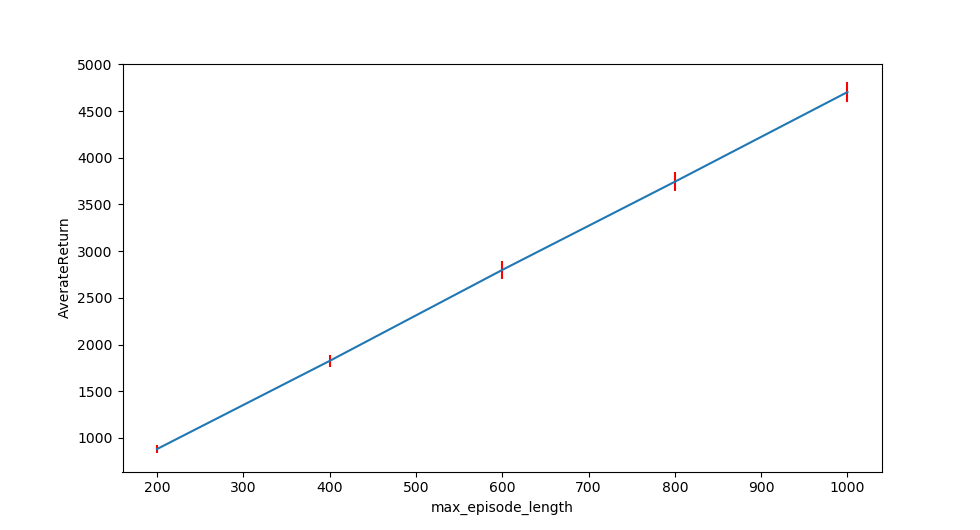
\includegraphics[width=.9\linewidth]{./Figure_1.png}
\caption{\label{Ablation}Ablation on the amount of data provided to BC, for \texttt{Ant-v2}.}
\end{figure}

We observe that the performance of the BC agent imporves linearly wrt the amount of data provided.

\clearpage
\section{Question 2.2}
\label{sec:org24f8b09}

\begin{table}[htbp]
\caption[DAgger for \texttt{Ant-v2}]{DAgger \textbf{\textbf{best results}} for \texttt{Ant-v2}.}
\centering
\begin{tabular}{l|r|r}
\texttt{Ant-v2} & DAgger & Expert\\
\hline
\texttt{AverageReturn} & 4764.02 & 4713.66\\
\hline
\texttt{StdReturn} & 116.59 & 12.20\\
\end{tabular}
\end{table}


\begin{table}[htbp]
\caption[DAgger for \texttt{Walker2d-v2}]{DAgger \textbf{\textbf{best results}} for \texttt{Walker2d-v2}.}
\centering
\begin{tabular}{l|r|r}
\texttt{Walker2d-v2} & DAgger & Expert\\
\hline
\texttt{AverageReturn} & 5588.88 & 5566.85\\
\hline
\texttt{StdReturn} & 29.49 & 9.24\\
\end{tabular}
\end{table}


\begin{table}[htbp]
\caption[DAgger for \texttt{Humanoid-v2}]{DAgger \textbf{\textbf{best results}} for \texttt{Humanoid-v2}.}
\centering
\begin{tabular}{l|r|r}
\texttt{Humanoid-v2} & DAgger & Expert\\
\hline
\texttt{AverageReturn} & 324.12 & 10344.52\\
\hline
\texttt{StdReturn} & 69.96 & 20.99\\
\end{tabular}
\end{table}

\begin{itemize}
\item Observation: DAgger significanly helps in the case of \texttt{Walker2d-v2}, and actually cracks the task. Moreover, the performance variance is reduced significantly via DAgger.

\item Obervation: DAgger fails to improve the performance in the case of \texttt{Humanoid-v2}.

\begin{figure}[htbp]
\centering
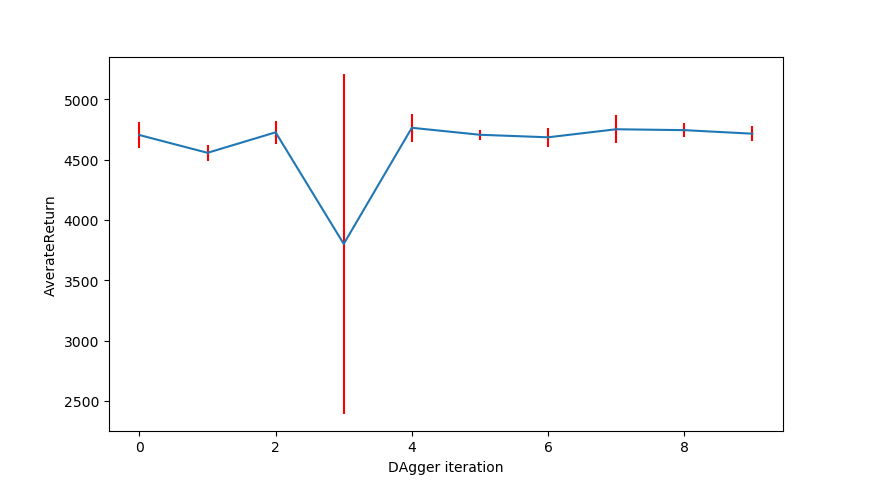
\includegraphics[width=.9\linewidth]{./Figure_2.png}
\caption{DAgger performance for \texttt{Ant-v2}.}
\end{figure}
\end{itemize}


\begin{figure}[htbp]
\centering
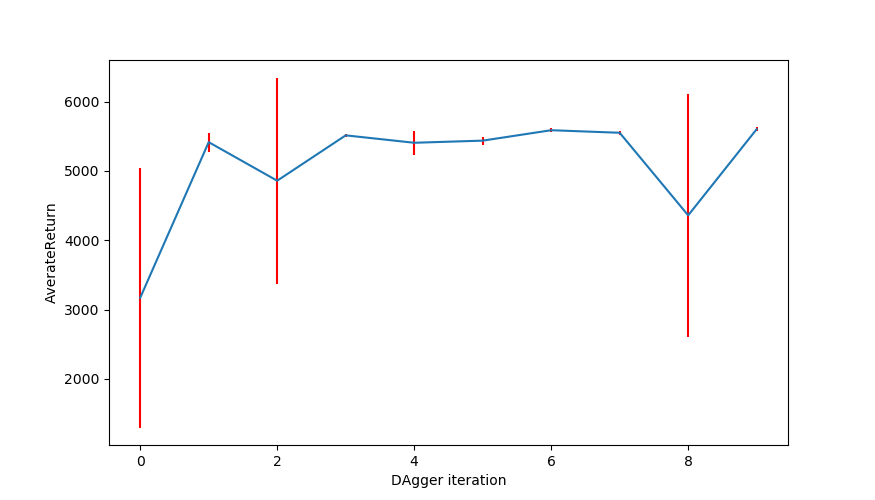
\includegraphics[width=.9\linewidth]{./Figure_3.png}
\caption{DAgger performance for \texttt{Walker2d-v2}.}
\end{figure}

\begin{itemize}
\item Note: The variance, i.e. error bars, seem to be large for some data points, and that is because we are using 5 trajectories during evaluation which is a small number. It was prescribed in the assignment, but I am now realizing we could benefit from a larger sample size.
\end{itemize}
\end{document}
